\begin{align}
\vec{C} - \vec{A} = \myvec{
4\\
0
} \equiv 
\myvec{
1\\
0
},\,
\implies \phi= 0\degree
\end{align}
		where
$\phi$ is the angle made by $AC$ with the x-axis.
Also, the diagonal
\begin{align}
	d = \norm{\vec{C}-\vec{A}} = 4
\end{align}
\begin{enumerate}
	\item We start with  the square in \figref{fig:7/4/4/4Fig3},
 with vertices as columns of the matrix
\begin{align}
	\vec{y} = \frac{d}{\sqrt 2}\myvec{0 & 1 & 1 & 0 \\ 0 & 0 & 1 & 1}
\end{align}
	in \eqref{eq:conic_affine}.
\item The next square, obtained as 
\begin{align}
\vec{P}\vec{y},
\end{align}
which is a rotated version of 
\figref{fig:7/4/4/4Fig3},
is available in 
\figref{fig:7/4/4/4Fig2}.  The angle of rotation
\begin{align}
	\theta = \phi - \frac{\pi}{4}
\end{align}
\item The desired square  is obtained using
\eqref{eq:conic_affine} as
\begin{align}
	\vec{x}=\vec{P}\vec{y} + \myvec{\vec{A} & \vec{A} &\vec{A} &\vec{A}} = 
		\myvec{
-1  &1 & 3 & 1 \\
2 & 0 & 2 & 4
	}
\end{align}
and available in 
\figref{fig:7/4/4/4Fig1}. The 2nd and 4th columns in the above matrix are 
$\vec{B}$ and $\vec{C}$ respectively.
\end{enumerate}
\begin{figure}[H]
	\begin{center} 
	    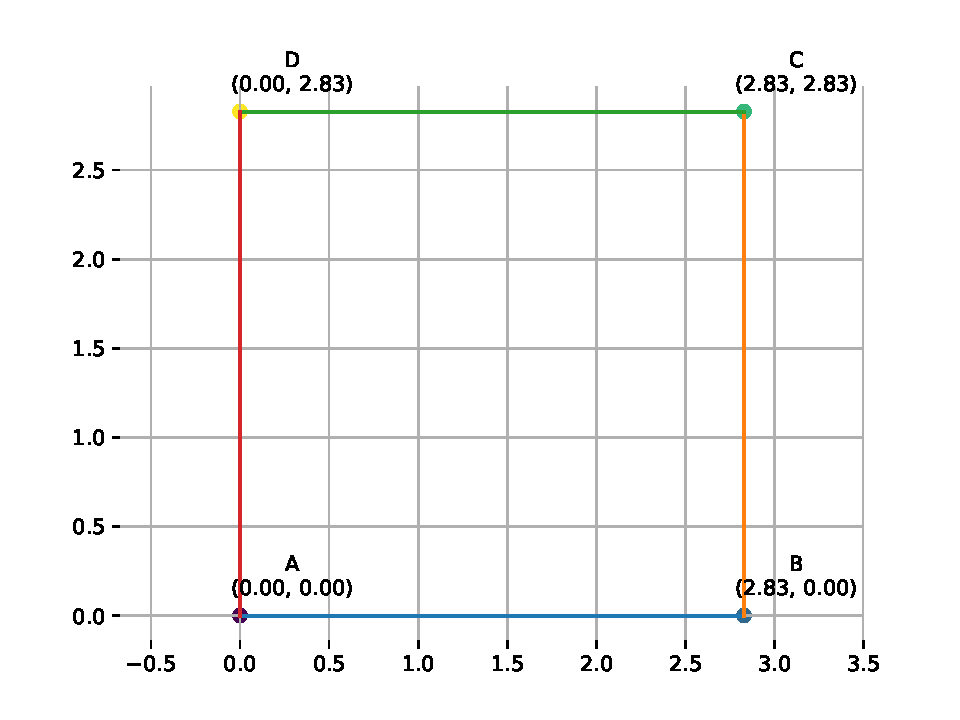
\includegraphics[width=0.75\columnwidth]{chapters/10/7/4/4/figs/fig.pdf}
	\end{center}
\caption{}
\label{fig:7/4/4/4Fig3}
\end{figure}
\begin{figure}[H]
	\begin{center} 
	    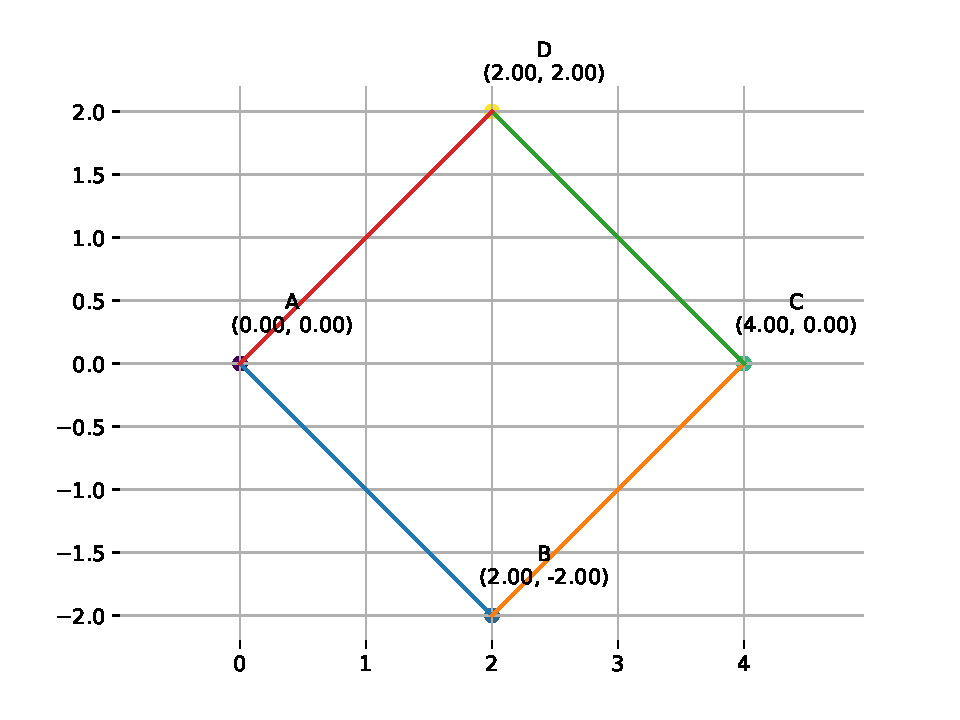
\includegraphics[width=0.75\columnwidth]{chapters/10/7/4/4/figs/fig1.pdf}
	\end{center}
\caption{}
\label{fig:7/4/4/4Fig2}
\end{figure}
\begin{figure}[H]
	\begin{center} 
	    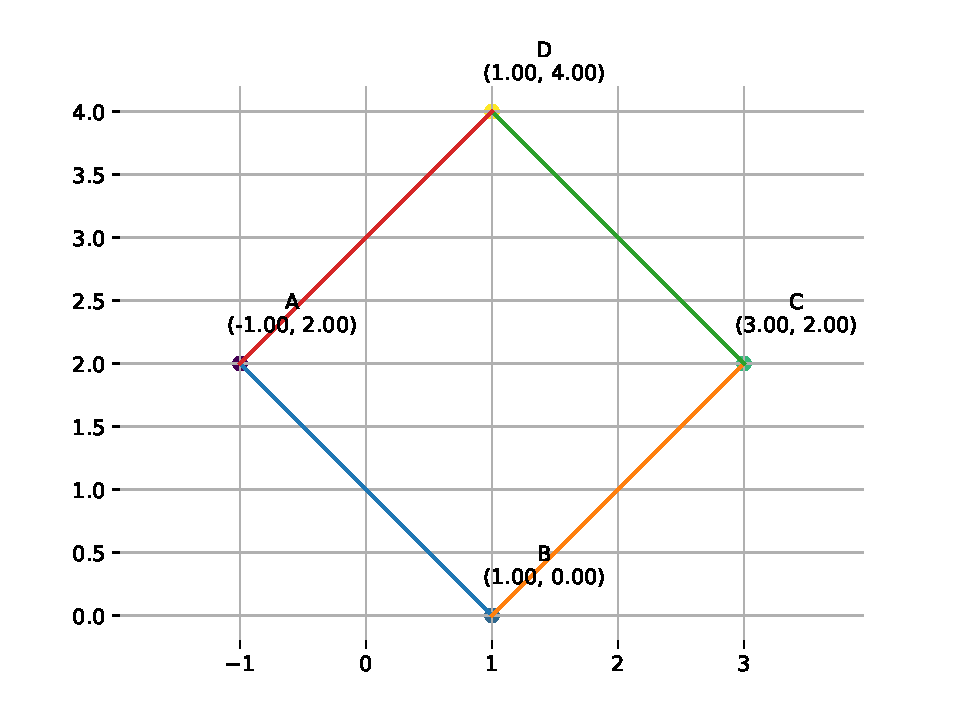
\includegraphics[width=0.75\columnwidth]{chapters/10/7/4/4/figs/fig2.pdf}
	\end{center}
\caption{}
\label{fig:7/4/4/4Fig1}
\end{figure}
